\documentclass{math}

\usepackage{tikz}

\title{Multivariable and Vector Calculus}
\author{Alvin Lin}
\date{August 2017 - December 2017}

\begin{document}

\maketitle

\section*{Review 2}
Arc Length:
\[ \int_{C}f\diff{S} = \int_{a}^{b}f|r'(t)|\diff{t} \]
\[ \int_{C_{AB}}\vec{F}\cdot\diff{r} = \int_{C}\vec{F}\cdot\vec{T}\diff{S} =
  \int_{a}^{b}\vec{F}\cdot\overrightarrow{r'(t)}\diff{t} \]
For \( r(u,v) \quad (u,v)\in D \):
\[ \iint_{S}f\diff{S} =
  \iint_{D}f\left|\pdiff{r}{u}\times\pdiff{r}{v}\right|\diff{u}\diff{v} \]
\[ \iint_{S}\vec{F}\cdot\diff{S} = \iint_{S}(\vec{F}\cdot\vec{r})\diff{S} =
  \iint_{D}\vec{F}\cdot\left(\pdiff{r}{u}\times\pdiff{r}{v}\right)
  \diff{u}\diff{v} \]
\[ \iint_{S}(\vec{\triangledown}\times\vec{F})\cdot\diff{S} =
  \iint_{S}\text{curl}~F\diff{S} =
  \iint_{D}(\vec{\triangledown}\times\vec{F})\cdot
  \left(\pdiff{r}{u}\times\pdiff{r}{v}\right)\diff{u}\diff{v} \]
Greene's Theorem:
\[ \iint_{D}Q_x-P_y\diff{A} \]

\subsubsection*{Example}
Compute the line integral:
\[ \int_{C}x\diff{S} \]
\( C \) is the curve \( y = x^2 \) from (0,0) to (1,1).
\begin{align*}
  \overrightarrow{r(t)} &= \langle t,t^2\rangle \\
  \overrightarrow{r'(t)} &= \langle1,2t\rangle \\
  \int_{C}x\diff{S} &= \int_{a}^{b}f|r'(t)|\diff{t} \\
  &= \int_{0}^{1}t\sqrt{1+4t^2}\diff{t}
\end{align*}

\subsubsection*{Example}
Compute the line integral:
\[ \int_{C}\langle y,x+y^2\rangle\cdot\diff{r} \]
\( C \) is the curve \( 4x^2+9y^2 = 36 \) in the counterclockwise orientation.
\begin{align*}
  \overrightarrow{r(t)} &=
    \left\langle\frac{6\cos(t)}{2},\frac{6\sin(t)}{3}\right\rangle \\
  \int_{C}\langle y,x+y^2\rangle\cdot\diff{r} &=
    \int_{0}^{2\pi}\langle2\sin(t),3\cos(t)+4\sin^2(t)\rangle\cdot
    \langle-3\sin(t),2\cos(t)\rangle\diff{t} \\
  &= \int_{0}^{2\pi}-6\sin^2(t)+6\cos^2(t)+8\sin^2(t)\cos(t)\diff{t} \\
\end{align*}
Using Greene's Theorem:
\begin{align*}
  \int_{C}\langle y,x+y^2\rangle\cdot\diff{r} &= \iint_{D}Q_x-P_y\diff{A} \\
  &= \iint_{D}1-1\diff{A} \\
  &= 0
\end{align*}

\subsubsection*{Example}
Find the work done along the curve \( C \) of the function:
\[ \int_{C}\langle2xy,x^2\rangle\cdot\diff{r} \]
given that the curve \( C \) is:
\begin{center}
  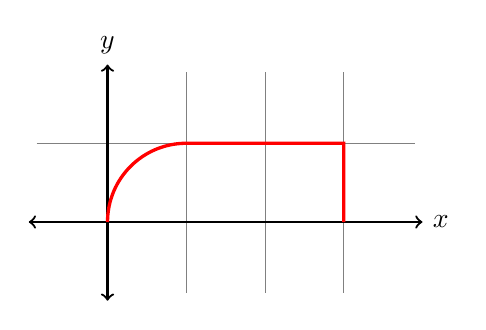
\begin{tikzpicture}
    \draw[step=1cm,gray,very thin] (-0.9,-0.9) grid (3.9,1.9);
    \draw[thick,<->] (-1,0) -- (4,0) node[right] {\( x \)};
    \draw[thick,<->] (0,-1) -- (0,2) node[above] {\( y \)};
    \draw[red, very thick] (0,0) arc (180:90:1) -- (3,1) -- (3,0);
  \end{tikzpicture}
\end{center}

\subsubsection*{Example}
Evaluate:
\[ \int_{C}\langle\e^y,x\e^y+\e^z,y\e^z\rangle\cdot\diff{r} \]
Given \( C \) is the line from (0,2,0) to (4,0,3).
\begin{align*}
  f_x &= \e^y \quad f = x\e^y+C_1(y,z) \\
  f_y &= x\e^y+\e^z \quad f = x\e^y+y\e^z+C_2(x,z) \\
  f_z &= y\e^z \quad f = y\e^z+C_3(x,y) \\
  f &= x\e^y+y\e^z \\
  \int_{C}\langle\e^y,x\e^y+\e^z,y\e^z\rangle\cdot\diff{r} &=
    \int_{(0,2,0)}^{(4,0,3)}x\e^y+y\e^z\diff{x}\diff{y}\diff{z}
\end{align*}

\subsubsection*{Example}
Give the parameterization of the region bounded by:
\[ x^2+y^2+z^2 = 10 \quad z = 1 \quad z = 3 \]
\[ \overrightarrow{r(R,\theta)} =
  \langle R\cos\theta,R\sin\theta,\sqrt{10-R^2}\rangle \quad
  1\le R\le 3 \quad 0\le\theta\le2\pi \]

\subsubsection*{Example}
Find the surface area of the region bounded by:
\[ z = \sqrt{x^2+y^2} \quad y = x \quad y = x^2 \]
\begin{align*}
  \overrightarrow{r(x,y)} &= \langle x,y,\sqrt{x^2+y^2}\rangle \\
  \iint_{S}1\diff{S} &= \int_{0}^{1}\int_{x^2}^{x}
    \left|\pdiff{r}{u}\times\pdiff{r}{v}\right|\diff{x}\diff{y}\diff{x} \\
  &= \int_{0}^{1}\int_{x^2}^{x}\begin{vmatrix}
    \i & \j & \k \\
    1 & 0 & \frac{2x}{2\sqrt{x^2+y^2}} \\
    0 & 1 & \frac{2y}{2\sqrt{x^2+y^2}}
  \end{vmatrix}\diff{y}\diff{x} \\
  &= \int_{0}^{1}\int_{x^2}^{x}
    \sqrt{\frac{x^2}{x^2+y^2}+\frac{y^2}{x^2+y^2}+1}\diff{y}\diff{x} \\
  &= \int_{0}^{1}\int_{x^2}^{x}\sqrt{2}\diff{y}\diff{x}
\end{align*}

\subsubsection*{Example}
Evaluate:
\[ \iint_{S}\langle x^2,xy,z\rangle\cdot\diff{S} \]
where \( S \) is bounded by \( z = x^2+y^2 \) below \( z = 1 \) with upwards
orientation.
\begin{align*}
  \overrightarrow{r(R,\theta)} &= \langle R\cos\theta,R\sin\theta,R^2\rangle \\
  \left|\pdiff{r}{R}\times\pdiff{r}{\theta}\right| &= \begin{vmatrix}
    \i & \j & \k \\
    \cos\theta & \sin\theta & 2R \\
    -R\sin\theta & R\cos\theta & 0
  \end{vmatrix} \\
  &= \langle-2R^2\cos\theta-2R^2\sin\theta,R\rangle \\
  \iint_{S}\langle x^2,xy,z\rangle\cdot\diff{S} &=
    \int_{0}^{2\pi}\int_{0}^{1}\langle R^2\cos^2\theta,R^2\sin\theta\cos\theta,
    R^2\rangle\cdot\left|\pdiff{r}{R}\times\pdiff{r}{\theta}\right|
    \diff{R}\diff{\theta} \\
  &= \int_{0}^{2\pi}\int_{0}^{1}-2R^4\cos^3\theta-4R^4\sin^2\theta\cos\theta+
    R^3\diff{R}\diff{\theta}
\end{align*}

\begin{center}
  You can find all my notes at \url{http://omgimanerd.tech/notes}. If you have
  any questions, comments, or concerns, please contact me at
  alvin@omgimanerd.tech
\end{center}

\end{document}
